% !TeX spellcheck = en_US
\addsection{Setup}{\skills/necromancy.png}

\begin{multicols*}{2}

This section will guide you through the process of setting up a Scenario from the Mission Book.

\begin{enumerate}
  \item Select a Scenario from the Mission Book.
    For your first game, we recommend choosing the "Brave New World" Scenario (see page 7 in the Mission Book).
  \item Choose your Faction from those available.
  \item Choose one of your Faction's Heroes as your Main Hero.
    Each Faction has at least one double-sided Hero Card, with each side depicting a different Hero.
  \item Take the following components belonging to your Faction:
  \begin{itemize}
    \item[a)]1 × Double-sided Hero Card (on the side of the chosen Hero)
    \item[b)]2 × Hero model
    \item[c)]7 × Town Building Tile
    \item[d)]1 × Town Board
    \item[e)]7 × Double-sided Unit Card
    \item[f)]3 × Hero-specific Specialty Card (of the chosen Hero)
    \item[g)]1 × Hero-specific Ability Card (of the chosen Hero)
    \item[h)]20 × Faction Cube
    \item[i)]1 × Build Token
    \item[j)]1 × Population Token
    \item[k)]1 × Spell Book Token
    \item[l)]3 × Movement Tokens
  \end{itemize}
  \item Place one of your Faction Cubes on the first space of the Level Tracker found on the Hero Card (Represented by a "1").
    Your hero is now Level 1.
  \item Set up the Map Tiles and other Scenario-specific components as shown in the Mission Book.
  \item Place the Town Board of your chosen Faction in front of you and set the Town Building Tiles next to it.
    Check which Buildings are already built in the Scenario you are about to play, and place the respective Building Tiles on the Town Board.
    Resolve any immediate effects from already built Buildings at the end of the setup.
  \item Set your starting income as indicated by the Scenario by placing your Faction Cubes on the income trackers on your Town Board.
    Place the Population, Build, and Spell Book Tokens in their respective slots on the Town Board.
  \item Group the Resource Tokens into separate piles located within reach of all players.
    Take the starting Resources determined by the Scenario you are playing and place them next to your Town Board.
    This is your Resource pool.
  \item Separate the remaining Tokens into their respective piles.
  \item Sort the Statistic Cards into four piles: Attack, Defense, Power, and Knowledge.
    Refer to the Statistics on your \hyperlink{Herocard}{Hero Card} and take the corresponding number of Cards from each pile.
  \item If your Main Hero is a Hero of Might \includesvg[height=10px]{\svgs/might.svg}, add 1 copy of the Magic Arrow Spell to Your Deck, and if they’re a Hero of Magic \includesvg[height=10px]{\svgs/magic.svg}, add 2 of these Spells to Your Deck.
  \item Add your Hero's \hyperlink{Ability}{Ability} and Level 1 \hyperlink{Specialty}{Specialty} Cards to your Starting Deck.
  \item Shuffle your Starting Deck and place it face down next to your Hero Card.
    This Deck is your Main Hero's \textbf{Deck of Might \& Magic}\index{Deck of Might \& Magic}, and is now ready. In this rule book, this is shortened to \textbf{Your Deck}.
  \item Sort the Ability, Artifact, and Spell Cards into 3 face down Decks (including any unused Magic Arrow Spells) and shuffle them.
    From each of these Decks, take the top Card and place it face up next to its Deck, creating 3 separate Discard Piles.
  \item Choose the Scenario's \hyperlink{Difficulty}{Difficulty} and take the corresponding Starting Bonus(es).
  \item Sort the Neutral Units into 4 Decks according to their tier (\includesvg[height=10px]{\svgs/bronze.svg}\includesvg[height=10px]{\svgs/silver.svg}\includesvg[height=10px]{\svgs/golden.svg}\includesvg[height=10px]{\svgs/azure.svg}).
    Shuffle these Decks and leave enough room for their Discard Piles.
  \item Place the Combat Board within reach of the players.
    Check the Scenario for which starting Units you receive and place them into a pile near your Town Board, separate from the rest of your Faction’s Units.
  \item Place the Round Tracker next to the game map and place a Black Cube on the "1" space.
  \item Shuffle the Astrologers Proclaim Cards and place them face down next to the Round Tracker.
  \item Orientate your Starting Tile to your liking.
    Choose which Hero model represents your Main Hero in this game and place the chosen model on the center Field of your Starting Tile.
  \item Choose a starting player. The starting player never changes during the game.
\end{enumerate}

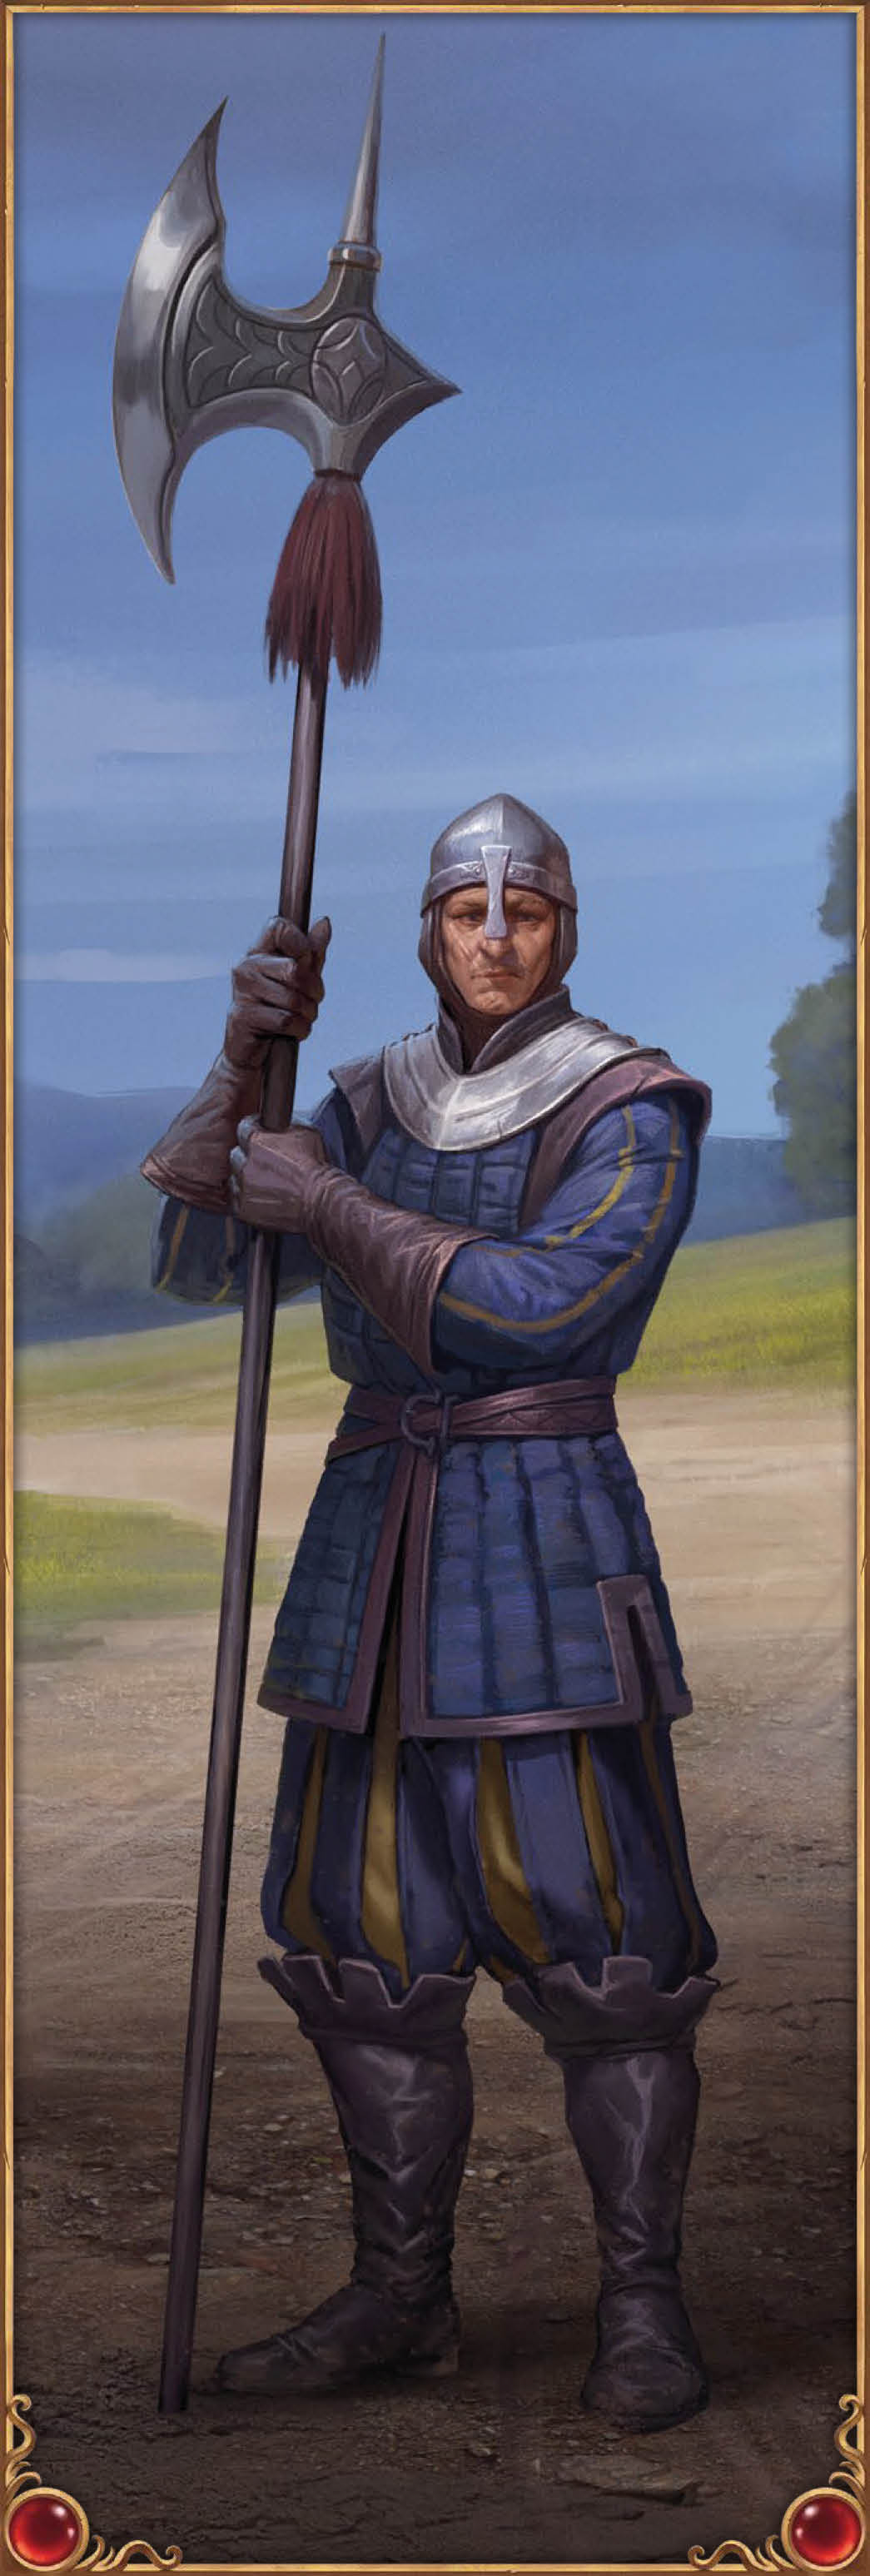
\includegraphics[width=\linewidth]{\art/halberdier.jpg}

\vspace*{\fill}

\end{multicols*}

\begin{figure}[h]
  \centering
  \begin{scriptsize}
  \begin{tikzpicture}
    \draw (0, 0) node[inner sep=0] {\makebox[\textwidth][c]{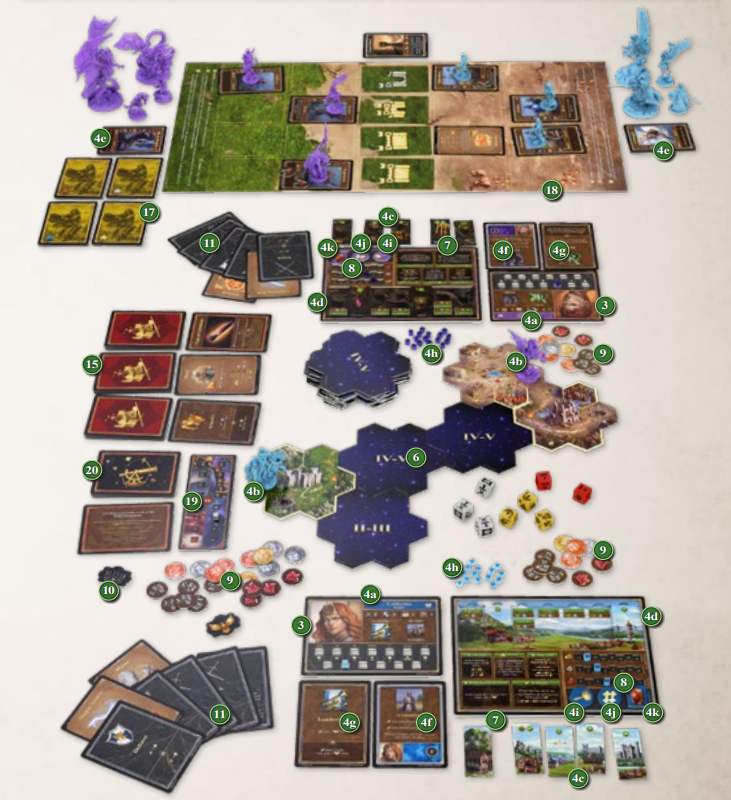
\includegraphics[width=1.25\linewidth]{\images/setup.png}}};
    \draw (6.2, 2.9) node {\encircle{\phantom{.}3\phantom{.}}};
    \draw (-1.8, -5.5) node {\encircle{\phantom{.}3\phantom{.}}};
    \draw (0, -4.7) node {\encircle{4a}};
    \draw (4.3, 2.4) node {\encircle{4a}};
    \draw (-3.1, -1.7) node {\encircle{4b}};
    \draw (3.9, 1.4) node {\encircle{4b}};
    \draw (5.5, -9.6) node {\encircle{4c}};
    \draw (0.5, 5.2) node {\encircle{4c}};
    \draw (7.3, -5.5) node {\encircle{4d}};
    \draw (-1.3, 2.9) node {\encircle{4d}};
    \draw (-7.1, 7.5) node {\encircle{4e}};
    \draw (7.5, 7) node {\encircle{4e}};
    \draw (1.3, -7.9) node {\encircle{4f}};
    \draw (3.7, 4.4) node {\encircle{4f}};
    \draw (-0.5, -7.9) node {\encircle{4g}};
    \draw (5, 4.4) node {\encircle{4g}};
    \draw (1.6, 1.7) node {\encircle{4h}};
    \draw (1.9, -4.3) node {\encircle{4h}};
    \draw (5.5, -7.9) node {\encircle{4i}};
    \draw (0.5, 4.4) node {\encircle{4i}};
    \draw (6.3, -7.9) node {\encircle{4j}};
    \draw (-0.1, 4.4) node {\encircle{4j}};
    \draw (7.3, -7.9) node {\encircle{4k}};
    \draw (-1.2, 4.5) node {\encircle{4k}};
    \draw (2.6, 2.0) node {\encircle{4l}};
    \draw (7.0, -4.3) node {\encircle{4l}};
    \draw (1.4, -1.3) node {\encircle{\phantom{.}6\phantom{.}}};
    \draw (3.1, -8.1) node {\encircle{\phantom{.}7\phantom{.}}};
    \draw (2.2, 4.4) node {\encircle{\phantom{.}7\phantom{.}}};
    \draw (6.5, -6.9) node {\encircle{\phantom{.}8\phantom{.}}};
    \draw (-0.5, 3.8) node {\encircle{\phantom{.}8\phantom{.}}};
    \draw (-3.1, -4.5) node {\encircle{\phantom{.}9\phantom{.}}};
    \draw (6.3, -3.6) node {\encircle{\phantom{.}9\phantom{.}}};
    \draw (6.1, 1.6) node {\encircle{\phantom{.}9\phantom{.}}};
    \draw (-6.6, -4.5) node {\encircle{10}};
    \draw (-4, 4.5) node {\encircle{11}};
    \draw (-4, -7.5) node {\encircle{11}};
    \draw (-7.1, 1.5) node {\encircle{15}};
    \draw (-5.6, 5.5) node {\encircle{17}};
    \draw (5.1, 5.8) node {\encircle{18}};
    \draw (-4.8, -2) node {\encircle{19}};
    \draw (-7.1, -1.5) node {\encircle{20}};
  \end{tikzpicture}
  \end{scriptsize}
\end{figure}
